
\newif\ifvimbug
\vimbugfalse

\ifvimbug
\begin{document}
\fi

\exercise{Reinforcement Learning}

You recently acquired a robot for cleaning you apartment but you are not happy with its performance and you decide to reprogram it using the latest AI algorithms. As a consequence the robot became self-aware and, whenever you are away, it prefers to play with toys rather than cleaning the apartment. Only the cat has noticed the strange behavior and attacks the robot. The robot is about to start its day and its current perception of the environment is as following 
%
\begin{center}
	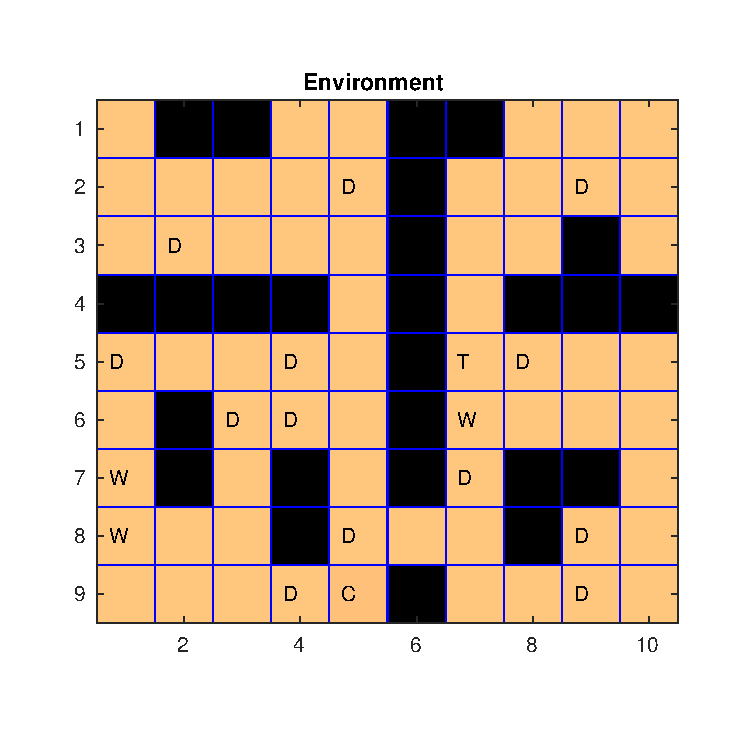
\includegraphics[width=0.75\textwidth]{gridworld.pdf}
\end{center}
%
The black squares denote extremely dangerous states that the robot must avoid to protect its valuable sensors. The reward of such states is set to $r_\textrm{danger}=-10^5$ (NB: the robot can still go through these states!). Moreover, despite being waterproof, the robot developed a phobia of water (W), imitating the cat. The reward of states with water is $r_\textrm{water}=-100$. The robot is also afraid of the cat (C) and tries to avoid it at any cost. The reward when encountering the cat is $r_\textrm{cat}=-3000$. The state containing the toy (T) has a reward of $r_\textrm{toy}=1000$, as the robot enjoys playing with them. Some of the initial specification still remain, therefore the robot receives $r_\textrm{dirt}=35$ in states with dirt (D).

State rewards can be collected at every time the robot is at that state. 
The robot can perform the following actions: \textit{down, right, up, left} and
\textit{stay}.

In our system we represent the actions with the an ID (0, 1, 2, 3, 4), while the grid is indexed as $\{ \texttt{row}, \texttt{column} \}$. The robot can't leave the grid as it is surrounded with walls.
A skeleton of the gridworld code and some plotting functions are available at the webpage.
For all the following questions, always attach a snippet of your code.


\begin{questions}

\begin{question}{Finite Horizon Problem}{14}
In the first exercise we consider the finite horizon problem, with horizon $T=15$ steps.
The goal of the robot is to maximize the expected return 
\begin{equation}
J_\pi = \mathbb{E}_\pi\left[\sum_{t=1}^{T-1}r_t(s_t,a_t)+r_T(s_T)\right], \label{Eq:J}
\end{equation}
according to policy $\pi$, state $s$, action $a$, reward $r$, and horizon $T$. Since rewards in our case are independent of the action and the actions are deterministic, Equation~\eqref{Eq:J} becomes
\begin{equation}
J_\pi = \sum_{t=1}^{T}r_t(s_t).
\end{equation}
Using the Value Iteration algorithm, determine the optimal action for each state when the robot has 15 steps left. Attach the plot of the policy to your answer and a mesh plot for the value function. Describe and comment the policy: is the robot avoiding the cat and the water? Is it collecting dirt and playing with the toy? With what time horizon would the robot act differently in state $(9,4)$?

\begin{answer}
	

\noindent\begin{minipage}{.5\textwidth}
	\centering
	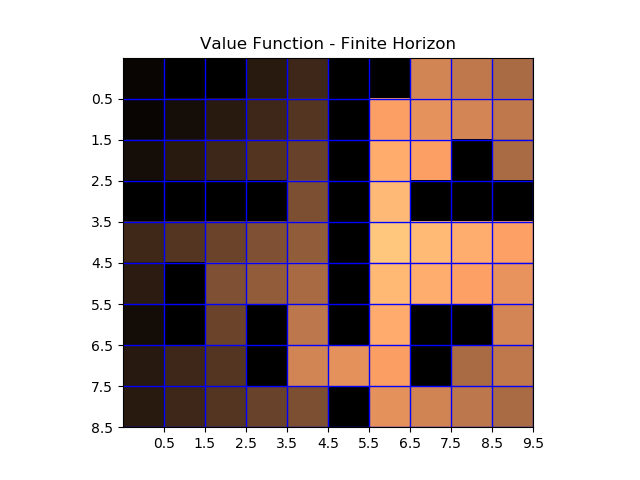
\includegraphics[width=1\textwidth]{img/value_2a.png} 
	\captionof{figure}{T=15, finite horizon Value Function}
	\label{fig:2a1}            
\end{minipage}%
\begin{minipage}{.5\textwidth}
	\centering
	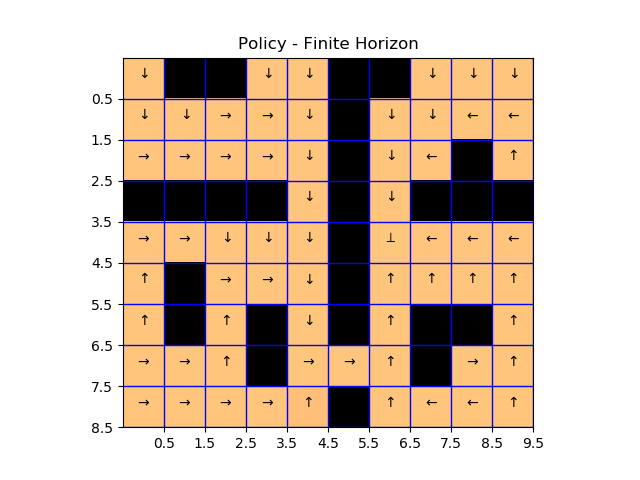
\includegraphics[width=1\textwidth]{img/policy_2a.png} 
	\captionof{figure}{T=15, finite horizon Policy}
	\label{fig:2a2}               
\end{minipage}
\begin{minipage}{.5\textwidth}
	\centering
	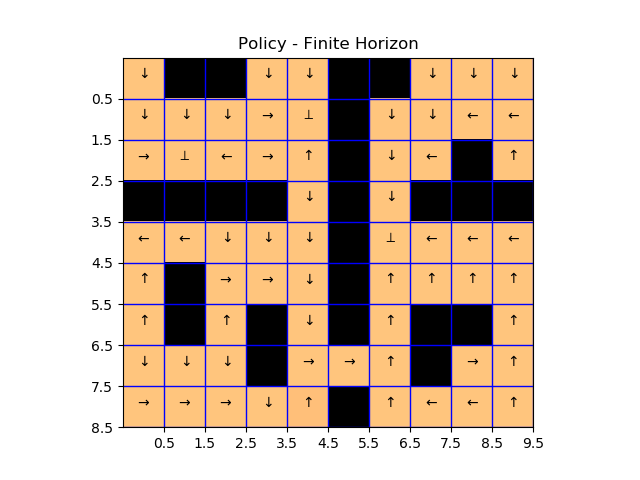
\includegraphics[width=1\textwidth]{img/2a_T10.png} 
	\captionof{figure}{T=10, finite horizon Policy}
	\label{fig:2a3}               
\end{minipage}

Policy of the robot:\\
The robot is trying to avoid the water and the cat(for T=15) if possible (see for example state(8,1) the robot is not moving to state 7,1 as this state is punished cause of its water). The robot is moving from all start states to the max. reward position (the toy at 5,7) avoiding all dangerous states. Thereby the robots is not so afraid of small punishments by the cat or water and moves also over these fields in order to reach the toy!

For T=10 the robot is moving differently and trying to avoid to move over the Cat's state at 9,4 (see Figure \ref{fig:2a3}).
	
\end{answer}

\end{question}

%----------------------------------------------


\begin{question}{Infinite Horizon Problem - Part 1}{4}
We now consider the infinite horizon problem, where $T=\infty$. Rewrite Equation~\eqref{Eq:J} for the infinite horizon case adding a discount factor $\gamma$. Explain briefly why the discount factor is needed.

\begin{answer}
Theory: \\
In the infinite time horizon case (when you live forever), the time index is not part of the state.  The optimal policy is time-independent: $\pi_t^*(a|s)=\pi^*(a|s)$. The reward and the transition model can no longer be time-dependent. There is a single stationary value function for all times. There are two different approaches to learning:
\begin{itemize}
	\item Value Iteration: Same as before just choose a large T for which the value function converges
	\item Policy Iteration: Learn a value function for the current policy. Update this policy and learn a new value function. Repeat.
\end{itemize}
Optimal policy for infinite horizon: $\pi^*=argmax_\pi J_\pi, \quad J_\pi=\sum_{t=0}^\infty \gamma^t r(s_t, a_t)$

In this case here:\\
\begin{equation}
J_\pi = \sum_{t=1}^{\infty} \gamma^t r_t(s_t).
\end{equation}

The discount factor $0<=\gamma<1$ trades-off long term vs. immediate reward. Without a discount factor many or all policies have infinite expected reward. For this reason a discount factor is required. Thereby future rewards $r_t(s,a)$ are discounted by $\gamma$ per time step.

	
\end{answer}

\end{question}

%----------------------------------------------


\begin{question}{Infinite Horizon Problem - Part 2}{6}
Calculate the optimal actions with the infinite horizon formulation. Use a discount factor of $\gamma=0.8$ and attach the new policy and value function plots.
What can we say about the new policy? Is it different from the finite horizon scenario? Why?

\begin{answer}
\noindent\begin{minipage}{.5\textwidth}
	\centering
	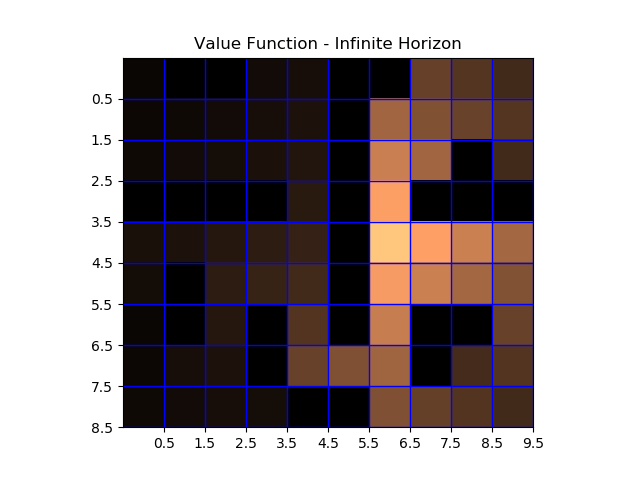
\includegraphics[width=1\textwidth]{img/infinitehorizon_2c.png} 
	\captionof{figure}{T=100, gamma=0.8 infinite horizon Value Function}
	\label{fig:2c1}            
\end{minipage}%
\begin{minipage}{.5\textwidth}
	\centering
	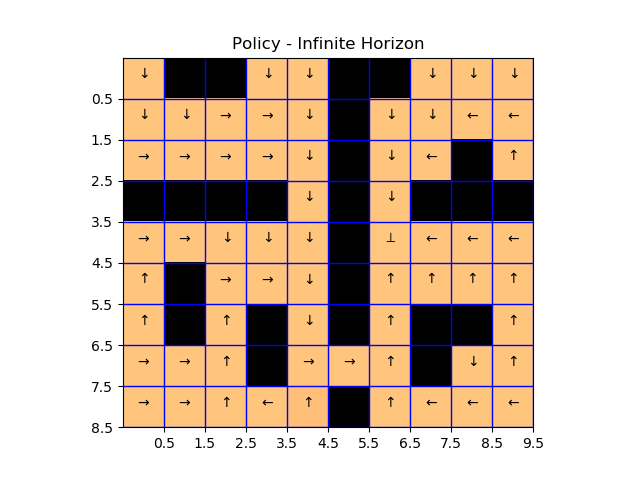
\includegraphics[width=1\textwidth]{img/policy_2c.png} 
	\captionof{figure}{T=100, gamma=0.8, infinite horizon Policy}
	\label{fig:2c2}               
\end{minipage}
\end{answer}

If the robot lives forever it avoids the cat to reach the toy! This is the only huge difference compared to the finite horizon scenario.

\end{question}

%----------------------------------------------


\begin{question}{Finite Horizon Problem with Probabilistic Transition Function}{10}
After a fight with the cat, the robot experiences control problems. 
For each of the actions \textit{up, left, down, right}, the robot has now a probability $0.7$ of correctly performing it and a probability of $0.1$ of performing another action according to the following rule: if the action is \textit{left} or \textit{right}, the robot could perform \textit{up} or \textit{down}. If the action is \textit{up} or \textit{down}, the robot could perform \textit{left} or \textit{right}.
Additionally, the action can fail causing the robot to remain on the same state with probability $0.1$.
Using the finite horizon formulation, calculate the optimal policy and the value function. Use a time horizon of $T=15$ steps as before. Attach your plots and comment them: what is the most common action and why does the learned policy select it?

\begin{answer}
	\begin{answer}
		\noindent\begin{minipage}{.5\textwidth}
			\centering
			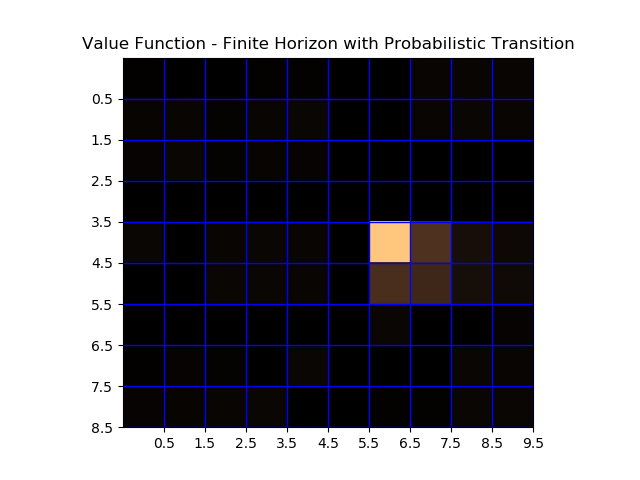
\includegraphics[width=1\textwidth]{img/value_2d.png} 
			\captionof{figure}{T=15, finite horizon Value Function}
			\label{fig:2d1}            
		\end{minipage}%
		\begin{minipage}{.5\textwidth}
			\centering
			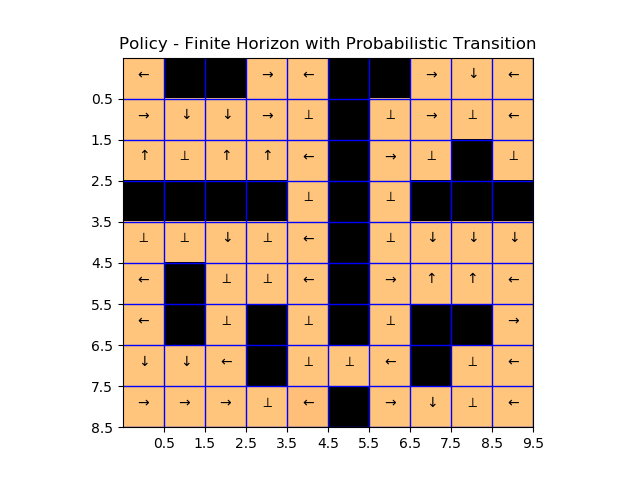
\includegraphics[width=1\textwidth]{img/policy_2d.png} 
			\captionof{figure}{T=15, finite horizon Policy}
			\label{fig:2d2}               
		\end{minipage}
	\end{answer}
	
\end{answer}

One of the more common action's is to stay at a reward position not risking a wrong movement to a punished position. One example is the state at 9,4. At this position the robot does not risk to move wrong in the right direction (into the cat). The learned policy rather let's the robot wait at a certain position than risking to move wrong into a punished state. One reason for that is the quite high probability of moving wrong (0.1).

\end{question}

%----------------------------------------------


\begin{question}[bonus]{Reinforcement Learning - Other Approaches}{8}
What are the two assumptions that let us use the Value Iteration algorithm? What if they would have been not satisfied? Which other algorithm would you have used? Explain it with your own words and write down its fundamental equation.

\begin{answer}
Some Theory:\\
Reinforcement Learning:\\
Contains a bunch of methods of machine learning. An agent(robot) learns a policy (Strategie) in order to increase its reward(Belohnung). At some particular states the agent get's a reward. With the knowledge of these rewards the agent optimizes a cost-function in order to learn the its optimal actions to increase its reward.

TD-Learning:\\
Temporal Difference Learning is a method of reinforcement learning. Compared to reinforcement learning the agent adapts after each action its policy according to an estimated reward. In reinforcement learning the agent adapts its policy after it collected some rewards in order to maximize its rewards. 


Value Iteration Assumptions:\\
Assume that the agent(robot) accurately knows the transition function(How the robot can move at each state? TODO ) and the reward(R matrix) for all states in the environment. This knowledge however can be learned with a method called Q-Learning.

Q-Learning:\\
Q-Learning is a specific method of TD-Learning in reinforcement learning. 
Q-learning is a form of model-free learning, meaning that an agent does not need to have any model of the environment; it only needs to know what states exist and what actions are possible in each state.
The way this works is as follows: we assign each state an estimated value, called a Q-value. When we visit a state and receive a reward, we use this to update our estimate of the value of that state. (Since our rewards might be stochastic, we may need to visit a state many times.)

Our Q-value can be written as:
\begin{equation}
Q(s,a)=R(s,a)+\gamma max_{a'} Q(s',a')
\end{equation}
We can use this to update the Q-value of a state-action pair as a reward r is observed:
\begin{equation}
Q_{t+1}(s,a)=r+\gamma max_{a'} Q_t(s',a')
\end{equation}
We still have one problem left to solve, however. How should an agent choose which action to test? We are assuming that the agent is learing in an onlinefashion.
This means that it is interleaving learning and execution. This brings up a tradeoff: learning is costly; time that our agent spends making mistakes is time that cannot be spent performing correct actions. One the other hand, time is needed to learn, and some time spent making errors early on can lead to improved overall performance. Our intuition is as follows: In the early stages of execution, when little is known about the world, it is important to explore and try unknown actions. There
is a great deal to be gained from learning, and the agent does not have enough information to act well in any case. Later in its life, the agent may want to almost always choose the action that looks best; there is little information to be gained, and so the value of learning is negligible. We will model this with a function that assigns a probability of being chosen for each possible action in a given state. This function should tend to choose actions with higher Q values, but should sometimes select lower Q-value actions. The probability of selecting the highest Q-value action should increase over time. We will use a distribution known as a Boltzmann distribution to do this.

TODO: oder nimm formeln von wikipedia: https://de.wikipedia.org/wiki/Temporal\_Difference\_Learning
was ist mit SARSA??: 
\end{answer}
\end{question}


\end{questions}
